\section{Histoire d'IPv4}
\label{sec:hist}
% Daniel intro

Une forte demande de la part des universités et centres de recherche aux
Etats-Unis à donné lieu à la création et la mise en ouvre d'un nouveau concept
de réseau permettant d'interconnecter les différentes structures de façon
efficace afin de partager des informations, et d'autre part, de faire des
expérimentations sur les réseaux.
\\
En effet jusqu'à présent les réseaux informatiques utilisaient le même principe que les
réseaux téléphoniques: la commutation de circuits; ce qui n'était pas très 
efficace en terme de ressources et de matériel\footnote {
Dans un réseau à commutation de circuits chaque périphérique pouvaient utiliser
un seul lien à la fois (circuit). Lors d'une transmission un lien était réservé
pour toute la durée de la communication et rendait donc le périphérique
inutilisable pour d'autre transmission vers un différent destinataire (c'est le même
principe que celui des réseaux téléphoniques).
http://www.tcpipguide.com/free/t\_CircuitSwitchingandPacketSwitchingNetworks.htm .}.
\\
Le concept de réseau à paquets commuté a été inventé et mis en 
pratique durant les années 1960. D'abord elle a été mise en pratique dans le réseau du NPL (UK National Physical Laboratory)
puis dans celui de l'agence américaine ARPA ({\it Advanced Research Project Agency})
\footnote {http://www.livinginternet.com/i/iw\_packet\_inv.htm}.
\\
Dans un réseau à commutation de paquets ({\it Packet Switching}), la connection
entre deux machines n'est pas continue et les données sont réparties et
envoyées en plusieurs paquets.  L'abandon d'une connection continue a permit de
se passer de la monopolisation d'un lien (circuit) dédié, ce qui a apporté la
possibilité d'avoir simultanément plusieurs connections (envoyer et recevoir
des paquets vers différents destinataires, un peu comme une boite aux lettres). 
\\
Le réseau créé au sein de l'agence gouvernemental ARPA, baptisé ARPANET, est un
des premiers réseaux à fonctionner sur la base de paquets. Le principe de
communication par paquet repose sur la découpe des informations à transmettre en plus
petits paquets qui peuvent chacun prendre un chemin différent pour arriver à
destination.  Avant ARPANET, la communication réseau était basée sur la
communication par circuit électrique dont les informations étaient envoyées en
continue sur un seul lien. Dans ce sens ARPANET a posé la base à partir de 
laquelle Internet a été créé. 
\\
L'ARPA (aujourd'hui DARPA: {\it Defence Advanced Research Project Agency}) est
une agence de recherche créée par le département américain de la défense en
1957 afin de développer de nouvelles technologies à usage militaire. ARPANET,
a été conçu comme un réseau en étoile reliant plusieurs serveurs.
Chaque serveur est représenté comme un noeud et peut stocker, traiter des données ou servir de relais.
Ainsi, il existe plusieurs chemins pour accéder à un noeud et lorsqu'un d'eux
est hors service, il est toujours possible de rejoindre le destinataire
en passant par un autre chemin. En effet, une des caractéristiques les plus intéressantes
d'ARPANET a été une certaine robustesse: ARPANET ne dépendait pas d'un centre
névralgique qui aurait pu être détruit en cas d'attaque\footnote { Il faut par
contre noter que l'hypothèse qui affirme que ARPANET ait été construit dans le
but de créer un réseau résistant aux attaques nucléaires a été démystifié par
l'{\it Internet Society}:
http://www.internetsociety.org/internet/what-internet/history-internet/brief-history-internet
.}
\\
Ce réseau se développa pour arriver à 23 noeuds en 1971 et 111 en 1977.
Afin d'uniformiser ce réseau, Vint Cerf et Bob Kahn ont introduit la première
version du protocol TCP.  Historiquement, le protocole IP constituait la
partie de TCP qui s'occupait de la transmission en mode sans connection.
La transmission en mode sans connection permet l'échange de paquet sans que les
deux hôtes soient obligés d'établir une connection auparavant.
Cette version est ce qu'on aurait pu nommer l'IPv1 et elle est documentée dans
la RFC 675. Elle fut modifiée et publiée en 1977 et correspond à la
deuxième version de TCP (IPv2). 
\\
Le protocole TCP avait donc deux fonctions: il devait premièrement
permettre une transmission fiable d'informations entre deux hôtes, et en plus
servir de protocole de routage et de packaging (partie correspondante à IP).
Cependant, pour être cohérent avec le modèle en couche, qui différencie la fiabilité
(couche transport) et le routage (couche réseau), il fut décidé en 1978 de
diviser le protocole TCP en deux protocoles distincts.\footnote {
{\it "We are screwing up in our design of internet protocols by violating the
principle of layering. Specifically we are trying to use TCP to do two
things: serve as a host level end to end protocol, and to serve as an
internet packaging and routing protocol. These two things should be
provided in a layered and modular way. I suggest that a new distinct
internetwork protocol is needed, and that TCP be used strictly as a host
level end to end protocol." } - IEN 2 (Comments on Internet Protocol and TCP)
}.

\begin{figure}[h]
\centering
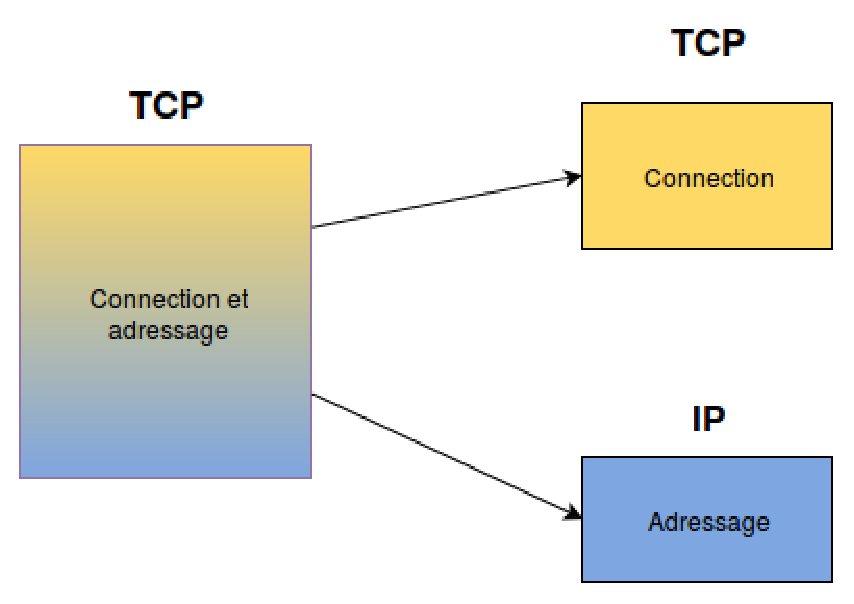
\includegraphics[width=7cm]{./pics/tcp2ip.eps}
\caption{Division de TCP en deux protocoles distincts.}
\label{fig:tcp2ip}
\end{figure}

Le protocole TCP ne s'occupe maintenant plus que de la partie transport. La
partie réseau a été prise en charge par le protocole IP.  C'est finalement le
1er janvier 1983 que l'ARPANET adopte les protocoles TCP et IP (IP dans sa version 4). 
